% Amidst experiment record (stage: D134 integration, 2026-11-08)
% Build: ./build.sh  (XeLaTeX + xeCJK). Every number carries a source tag [Sx];
% the source list is Appendix A. Do not add numbers without a GitHub/repo source.
\documentclass[11pt,a4paper]{article}

\usepackage{fontspec}
\usepackage[CJKmath=true]{xeCJK}
\setCJKmainfont[BoldFont={Songti TC Bold}]{Songti TC}
\setCJKsansfont{PingFang TC}
\setCJKmonofont{PingFang TC}
\setmainfont{Times New Roman}
\setsansfont{Helvetica Neue}
\setmonofont[Scale=0.85]{Menlo}
\xeCJKsetup{CJKspace=false}

\usepackage[margin=2.3cm]{geometry}
\usepackage{amsmath,amssymb}
\usepackage{graphicx}
\usepackage{booktabs,tabularx,array,multirow,longtable}
\usepackage{xcolor}
\usepackage{caption}
\usepackage{enumitem}
\usepackage{tikz}
\usetikzlibrary{arrows.meta,positioning,fit,calc,shapes.geometric,backgrounds}
\usepackage[hidelinks]{hyperref}
\usepackage{titlesec}

\captionsetup{font=small,labelfont=bf,labelsep=quad}
\renewcommand{\figurename}{圖}
\renewcommand{\tablename}{表}
\renewcommand{\contentsname}{目錄}
\renewcommand{\refname}{參考文獻}
\renewcommand{\abstractname}{摘要}
\renewcommand{\appendixname}{附錄}
\setlist{itemsep=2pt,topsep=3pt}
\linespread{1.25}
\sloppy
\setlength{\emergencystretch}{3em}
\titleformat{\section}{\large\bfseries\sffamily}{\thesection}{1em}{}
\titleformat{\subsection}{\normalsize\bfseries\sffamily}{\thesubsection}{1em}{}

% Source tag and status markers (grayscale-safe: text, not color)
\newcommand{\src}[1]{\textsuperscript{\scriptsize[#1]}}
\newcommand{\NR}{\texttt{NOT\_RUN}}
\newcommand{\UNK}{\texttt{UNKNOWN}}
\newcommand{\EXT}{\texttt{EXTRAPOLATED}}
\newcommand{\TBD}{\textbf{待補}}
\newcommand{\code}[1]{\texttt{\detokenize{#1}}}
\renewcommand{\eqref}[1]{Eq.~(\ref{#1})}

% TikZ styles: black/gray only, distinguish by line style and fill shade
\tikzset{
  box/.style={draw, rounded corners=2pt, align=center, font=\small, minimum height=8mm, inner sep=3pt, fill=white},
  off/.style={box, fill=black!8},
  ui/.style={box, fill=black!15},
  note/.style={font=\scriptsize, align=center},
  flow/.style={-{Stealth[length=2.2mm]}, thick},
  fb/.style={-{Stealth[length=2.2mm]}, thick, dashed},
  wall/.style={draw, very thick, dash dot},
}

\title{\sffamily\bfseries Amidst：Agentic 驅動之智慧監控數位孿生系統\\[4pt]
\large 階段實驗紀錄——多鏡頭查找與追蹤輔助（D134 整合版）}
\author{Amidst 專題小組\thanks{本紀錄由 Claude Code（Opus 5.5）依 GitHub 與 repo 內容整理；每個數字附來源標記 [S$n$]，對照附錄 A。}}
\date{2026 年 11 月 8 日}

\begin{document}
\maketitle

\begin{abstract}
\noindent 多鏡頭監控的視野彼此不重疊，目標走出一台鏡頭後會進入沒有任何鏡頭看得到的盲區，監控人員必須手動猜測下一台鏡頭。本紀錄整理 Amidst 在 D126 定位（「輔助、不求精確」）下的階段成果：系統只保留兩個核心功能——case1 查找（時間必填，地點或特徵至少一項）與 case2 追蹤（特徵必填，時間空白代表現在；自動換鏡頭，盲區在俯視圖以虛線畫出推測路線）。偵測以 RT-DETR R18 離線建立索引，展示時只查索引並重播，現場不跑模型。我們在 r004 與 r005 兩個場景、B-05／A4-1／B4-1 三個事件上完成功能驗收：後端 pytest 121 項、前端 Node 478 項（新 UI 分支 492 項）、合成瀏覽器 E2E 49 項、實機瀏覽器 E2E 53 項全數通過\src{S1,S2}。延遲方面，歷史量測顯示 RT-DETR 單 worker 為 3.129 fps，若要即時處理 9 台 5 fps 鏡頭約需 14.4 個 worker（\EXT）\src{S3}，支持「離線建索引、現場查詢」的設計；r004 上 2,050 張影格的離線偵測前向平均為 279.64 ms／張（3.576 fps）\src{S11}。我們也客觀檢討副標題中的「Agentic」：目前所有自主行為都是規則或演算法，語言模型 Agent 模式在歷史量測中 18 次全部逾時\src{S3}、預設關閉，因此「Agentic」尚未被實際驗證。研究問題 RQ3（自然語言理解）與 RQ4（2D 目標存在判斷）的正式結果待補。
\end{abstract}

\noindent\textbf{關鍵詞：}多鏡頭監控、不重疊視野、盲區推測、負證據、離線索引、跨鏡頭追蹤輔助、數位孿生

\tableofcontents
\newpage

%=====================================================================
\section{緒論}
\subsection{問題：多鏡頭之間的盲區}
室內監控通常由數台到數十台視野不重疊的鏡頭組成。目標在一台鏡頭消失後，可能經過走廊、轉角等沒有鏡頭的區域才在另一台鏡頭出現；這段時間內系統沒有任何觀測。主流多鏡頭多目標追蹤（MTMC）研究假設鏡頭經過校正、視野部分重疊，並以外觀重辨識輸出全域身分\cite{ristani2016,wang2024aic8,tang2025aic9}。實務上的監控人員更常需要的是：快速知道「某時段某地點有沒有符合條件的人」，以及「目標離開這台鏡頭後，下一台應該看哪裡」。

\subsection{定位：輔助、不求精確（D126）}
專案在 2026-11-04 的決策 D126 把核心收斂為兩項：查找與追蹤，其餘功能暫停。核心契約明訂系統是「輔助」：讓使用者快速知道目標大概在哪，不追求精確；所有輸出的身分判定一律為 \code{UNCONFIRMED}，串起來的片段是「條件相符的候選」，不是「同一個人」\src{S5}。證據狀態分為 \code{OBSERVED}、\code{INFERRED}、\code{MISSING}、\code{UNKNOWN} 四種，並在畫面上以不同線型區分\src{S5}。

\subsection{兩個核心功能}
\begin{itemize}
  \item \textbf{case1 查找}（API \code{q_core_search}）：時間範圍必填，地點或特徵（類別、顏色）至少填一項；回傳符合條件的鏡頭與時間片段，以結果牆呈現\src{S5}。
  \item \textbf{case2 追蹤}（API \code{q_core_track}）：特徵必填，時間空白代表「現在」；系統依單畫面切鏡規則自動換鏡頭，目標進入盲區時在俯視圖畫出推測虛線\src{S5}。
\end{itemize}

\subsection{貢獻}
\begin{enumerate}
  \item 一套「離線偵測建索引、現場查詢與重播」的查找／追蹤輔助架構，含 GT 隔離與 \code{RULE_ONLY} 退回路徑（第 \ref{sec:design} 節）。
  \item 以可達區域與「鏡頭有看但沒看到」負證據描述盲區推測的形式化定義（第 \ref{sec:blind} 節，\eqref{eq:reach}–\eqref{eq:admissible}）。
  \item 在兩個場景、三個事件上的功能驗收與自動化測試紀錄，每個數字附可追溯來源（第 \ref{sec:results} 節、附錄 A）。
  \item 對系統「Agentic」程度的客觀評估與補強計畫（第 \ref{sec:discussion} 節）。
\end{enumerate}

%=====================================================================
\section{相關研究}
本節依專題報告初稿第二章\src{S10}整理；初稿中尚未核對的書目欄位在參考文獻中保留「待核」。

\paragraph{多鏡頭多目標追蹤（MTMC）。}Ristani 等人提出以身分為核心的 IDF1 指標與 DukeMTMC 資料集\cite{ristani2016}。AI City Challenge 第 8、9 屆的人物追蹤賽道使用經校正的合成多鏡頭環境，以 3D 位置計算 HOTA\cite{wang2024aic8,tang2025aic9}。典型管線為偵測 → 單鏡頭追蹤 → ReID → 時空約束的跨鏡頭關聯 → 投影到 3D。

\paragraph{單鏡頭追蹤與重辨識。}ByteTrack 讓低分偵測框參與關聯\cite{zhang2022bytetrack}；BoT-SORT 加入鏡頭運動補償與可選 ReID\cite{aharon2022botsort}；OSNet 為輕量全尺度 ReID 骨幹\cite{zhou2019osnet}。這些方法輸出的是軌跡 ID 與外觀相似度，本質上是身分判斷。

\paragraph{多視角 3D 追蹤。}NVIDIA DeepStream MV3DT 要求鏡頭校正且視野重疊，以 3D 腳點跨鏡頭關聯\cite{nvidia_mv3dt}；WILDTRACK 以 7 台嚴格重疊、聯合校正的鏡頭拍攝同一空地\cite{chavdarova2018wildtrack}。

\paragraph{鏡頭拓撲與 camera link model。}與本研究最接近的脈絡。Kettnaker 與 Zabih 把不重疊鏡頭的路徑重建寫成貝氏問題\cite{kettnaker1999}；Javed 等人學習不重疊鏡頭間的時空與外觀關係\cite{javed2003}；Makris 等人非監督地學出出入口區與鏡頭連結\cite{makris2004}；Lee 等人線上估計含轉移時間的 camera link model\cite{lee_cltm}。共同點是「出入口區＋鏡頭連結」的圖結構。

\paragraph{自然語言影片檢索。}CityFlow-NL 以自然語言描述檢索車輛軌跡\cite{feng2021cityflownl}；CLIP4Clip 把 CLIP 用於文字—影片片段檢索\cite{luo2021clip4clip}；NVIDIA VSS Blueprint 結合 VLM、向量搜尋與 Agent 做片段檢索與摘要\cite{nvidia_vss}。

\paragraph{本研究定位。}Amidst 的鏡頭轉移圖與上述「出入口區＋鏡頭連結」屬同類結構，但圖由人工核准並在事件前凍結，不由資料學出；系統不輸出身分，因此不以 IDF1 或 HOTA 與 MTMC 方法比較精度\src{S10}。偵測器採用 RT-DETR\cite{lv2023rtdetr}。

%=====================================================================
\section{系統設計}\label{sec:design}
\subsection{系統架構}
圖~\ref{fig:arch} 為系統架構。上半為離線流程：影格先經 RT-DETR R18（\code{rtdetr_r18vd_dec3_6x_coco_from_paddle}，CPU、FP32、2 threads\src{S8}）偵測，結果寫入偵測索引；下半為線上流程：前台與後台經後端 API \code{q_core_search}／\code{q_core_track} 查詢索引、區域圖與鏡頭圖，再取回原始影格顯示\src{S5}。切鏡決策預設為 \code{RULE_ONLY}；語言模型 Agent（\code{AGENT_SEQUENTIAL}）失敗或逾時時退回規則（\code{RULE_FALLBACK}）\src{S7b}。物理預測服務未接上時，盲區欄位回 \code{UNAVAILABLE}，不捏造曲線\src{S5}。GT、渲染軌跡、visibility、depth 等一律不得進入推論與畫面；請求帶有這些鍵時回 422 \code{FORBIDDEN_INFERENCE_INPUT}\src{S5}。

\begin{figure}[htbp]
\centering
\begin{tikzpicture}[node distance=6mm and 7mm]
  % offline lane
  \node[off] (frames) {影格\\\scriptsize(PNG，r004/r005)};
  \node[off, right=of frames] (det) {離線偵測\\\scriptsize RT-DETR R18};
  \node[off, right=of det] (idx) {偵測索引\\\scriptsize\code{detection_index}};
  \node[off, right=of idx] (graphs) {區域圖／鏡頭圖\\\scriptsize(人工核准、pinned)};
  % online lane
  \node[box, below=16mm of idx, minimum width=58mm] (api) {後端 API\\\code{q_core_search} ／ \code{q_core_track}};
  \node[box, left=9mm of api] (rule) {切鏡決策\\\code{RULE_ONLY}（預設）};
  \node[box, below=7mm of rule] (agent) {Agent 模式\\\scriptsize Qwen3 1.7B（預設關閉）};
  \node[box, below=7mm of api] (blind) {盲區推測\\\scriptsize\code{INFERRED}，\code{DISPLAY_ONLY}};
  \node[ui, below=18mm of api, xshift=-22mm] (front) {前台\\\scriptsize 封面、case1／2／3};
  \node[ui, below=18mm of api, xshift=22mm] (admin) {後台\\\scriptsize 概況、設定};
  % GT
  \node[box, dashed, right=10mm of api, fill=black!4] (gt) {GT／渲染軌跡\\visibility／depth};
  % arrows
  \draw[flow] (frames) -- (det);
  \draw[flow] (det) -- (idx);
  \draw[flow] (idx) -- (api);
  \draw[flow] (graphs) |- (api);
  \draw[flow] (frames.west) -- ++(-4mm,0) coordinate (fl) |- (front.west) node[note, pos=0.25, left, align=right] {原始影格\\（顯示用）};
  \draw[flow] (api) -- (blind);
  \draw[flow] (rule) -- (api);
  \draw[fb] (agent.north) -- node[note, right] {逾時／失敗\\退回規則} (rule.south);
  \draw[flow] (api.south) ++(-20mm,0) -- (front);
  \draw[flow] (api.south) ++(20mm,0) -- (admin);
  \draw[very thick] ($(gt.west)+(-2mm,6mm)$) -- ($(gt.west)+(-2mm,-6mm)$);
  \node[note, below=1mm of gt] {GT 隔離：請求含此類鍵\\回 422 \code{FORBIDDEN_INFERENCE_INPUT}};
  % lanes
  \begin{scope}[on background layer]
    \node[draw, dotted, inner sep=4mm, fit=(frames)(graphs), label={[font=\scriptsize]above:離線（展示前完成）}] {};
    \node[draw, dotted, inner sep=4mm, fit=(rule)(agent)(api)(blind)(front)(admin), label={[font=\scriptsize]below:線上（展示時：只查索引與重播，不跑模型）}] {};
  \end{scope}
\end{tikzpicture}
\caption{系統架構。實線為資料流；虛線箭頭為 Agent 失敗時退回 \code{RULE_ONLY} 的路徑；右側虛線框與粗線表示 GT 類資料被隔離在推論之外。依據：核心契約\src{S5}、\code{q5_agent.py}\src{S7b}、r004 偵測設定\src{S8}。}
\label{fig:arch}
\end{figure}

\subsection{功能架構}
圖~\ref{fig:func} 為功能樹。前台由封面進入，三選一進入 case1 查找、case2 追蹤、case3 查看（事件重播）；後台有概況（狀態卡、偵測數據卡、各鏡頭偵測數、時間軸、事件流）與設定（只存在瀏覽器）\src{S2}。

\begin{figure}[htbp]
\centering
\begin{tikzpicture}[
  level distance=14mm,
  every node/.style={box, font=\scriptsize, minimum height=6mm},
  level 1/.style={sibling distance=80mm},
  level 2/.style={sibling distance=22mm, text width=16mm},
  every child node/.style={anchor=north},
  edge from parent/.style={draw, thick},
  edge from parent path={(\tikzparentnode.south) -- ++(0,-3mm) -| (\tikzchildnode.north)}]
  \node[ui] {Amidst 工作台}
    child { node[ui] {前台}
      child { node {封面} }
      child { node {case1 查找\\查詢窗\\結果牆} }
      child { node {case2 追蹤\\單／多畫面\\鏡頭時間軸\\俯視圖} }
      child { node {case3 查看\\事件列\\播放／倍速} }
    }
    child { node[ui] {後台}
      child { node {概況\\狀態卡\\偵測數據\\事件流} }
      child { node {設定\\（存在瀏覽器）} }
      child { node {鏡頭播放\\紀錄} }
    };
\end{tikzpicture}
\caption{功能架構（功能樹）。依據 PR \#487 描述\src{S2}。「鏡頭播放」「紀錄」為舊功能移入後台的分頁。}
\label{fig:func}
\end{figure}

\subsection{使用流程}
圖~\ref{fig:flow} 為使用流程。使用者從封面選擇 case，輸入條件後看到分段進度條；case1 結束於結果牆，case2 鎖定目標後依切鏡規則換鏡頭，目標離開所有鏡頭時進入盲區（俯視圖顯示推測虛線），若在等待期間沒有再被看到則標為跟丟（\code{LOST}）\src{S5,S2}。

\begin{figure}[htbp]
\centering
\begin{tikzpicture}[node distance=5mm and 6mm, every node/.append style={font=\scriptsize}]
  \node[ui] (cover) {封面};
  \node[box, right=of cover] (pick) {選 case};
  \node[box, right=of pick] (input) {輸入條件\\時間／地點／特徵};
  \node[box, right=of input] (prog) {進度條};
  \node[box, below=10mm of prog] (result) {case1：結果牆};
  \node[box, below=10mm of input] (lock) {case2：鎖定目標\\\code{ON_CAMERA}};
  \node[diamond, draw, aspect=2.2, inner sep=1pt, below=8mm of lock, align=center] (leave) {目標離開\\畫面？};
  \node[box, left=18mm of leave] (switch) {換鏡頭\\（規則 §3.5）};
  \node[box, below=8mm of leave] (blind) {盲區 \code{GAP}\\俯視圖推測虛線};
  \node[box, fill=black!25, right=24mm of blind] (lost) {跟丟 \code{LOST}};
  \draw[flow] (cover) -- (pick);
  \draw[flow] (pick) -- (input);
  \draw[flow] (input) -- (prog);
  \draw[flow] (prog) -- node[note, right] {case1} (result);
  \draw[flow] (prog.south west) -- node[note, above, sloped] {case2} (lock.north east);
  \draw[flow] (lock) -- (leave);
  \draw[flow] (leave) -- node[note, above] {他台看得到} (switch);
  \draw[flow] (switch) |- (lock);
  \draw[flow] (leave) -- node[note, right] {沒有鏡頭看到} (blind);
  \draw[flow] (blind) -- node[note, below] {等待後仍未出現} (lost);
  \draw[fb] (blind.west) -| node[note, below, pos=0.3] {再次被看到} (switch.south);
\end{tikzpicture}
\caption{使用流程。虛線表示盲區後重新取得觀測、接回切鏡流程。依據：核心契約 §3.5–3.6\src{S5}、PR \#487\src{S2}。}
\label{fig:flow}
\end{figure}

\subsection{盲區推測}\label{sec:blind}
目前整合版的 case2 盲區顯示走物理預測路徑：以最後觀測的腳點速度與出口區排序候選下一台鏡頭，並以名目路徑長度與速度範圍給出時間窗\src{S6}。設最後觀測時刻為 $t_s$，轉移的名目路徑長度為 $L$，速度範圍為 $[v_{\min}, v_{\max}]$（預設 $[0.5, 2.0]$ m/s，狀態為 PROPOSED，未核定\src{S6}），則候選鏡頭的出現時間窗為
\begin{equation}
  W = \left[\, t_s + \delta\,\frac{L}{v_{\max}},\;\; t_s + \frac{L}{v_{\min}} \,\right],
  \qquad \delta = \begin{cases} 0 & \text{兩鏡頭視野重疊 (OVERLAP)} \\ 1 & \text{其他} \end{cases}
  \label{eq:window}
\end{equation}
\eqref{eq:window} 只給時間，不給位置；俯視圖上的虛線只用靜態平面圖的顯示座標連線，信心一律為 \code{LOW}，用途為 \code{DISPLAY_ONLY}\src{S5}。

更完整的形式由 repo 中的盲區假設模組描述（\code{blind_hypothesis/engine.py}、\code{pruning.py}\src{S7}）。令可行走區域為 $\mathcal{M}$，$d_{\mathcal{M}}(\cdot,\cdot)$ 為 $\mathcal{M}$ 內的測地距離，盲區兩端的觀測位置與時刻為 $(x_s, t_s)$、$(x_e, t_e)$。時刻 $t \in [t_s, t_e]$ 的可達區域為前向與後向可達集合的交集：
\begin{equation}
  R(t) = \bigl\{\, x \in \mathcal{M} \;:\; d_{\mathcal{M}}(x_s, x) \le v_{\max}(t - t_s) \;\wedge\; d_{\mathcal{M}}(x, x_e) \le v_{\max}(t_e - t) \,\bigr\}.
  \label{eq:reach}
\end{equation}
負證據來自「鏡頭有看但沒看到」：若鏡頭 $c$ 在時刻 $t$ 有有效影格、其可見地面範圍為 $V_c(t)$，且偵測結果中沒有符合條件的目標，則目標在 $t$ 時不可能位於 $V_c(t)$。令 $\mathcal{N}(t)$ 為時刻 $t$ 提供負證據的鏡頭集合，未被看見的區域為
\begin{equation}
  U(t) = \mathcal{M} \setminus \bigcup_{c \in \mathcal{N}(t)} V_c(t),
  \label{eq:unseen}
\end{equation}
修剪後的可達區域為 $\tilde{R}(t) = R(t) \cap U(t)$。一條候選路線 $p:[t_s,t_e]\to\mathcal{M}$ 可被保留，若且唯若
\begin{equation}
  p(t_s)=x_s,\;\; p(t_e)=x_e,\;\; \|\dot p(t)\| \le v_{\max},\;\; p(t) \in \tilde{R}(t)\quad \forall t \in [t_s, t_e].
  \label{eq:admissible}
\end{equation}
新的負證據只能附加在既有證據之後；重跑時先前為 ACTIVE、但違反 \eqref{eq:admissible} 的路線被標為 \code{PRUNED} 並寫入修剪紀錄\src{S7}。排序依設定的合理程度，不是機率；身分維持 \code{UNCONFIRMED}，物理通行維持 \code{UNKNOWN}\src{S7}。此模組是否已接入整合版 case2 前台：\UNK（本紀錄未驗證），因此第 \ref{sec:results} 節的盲區畫面只對應 \eqref{eq:window} 的顯示路徑。

%=====================================================================
\section{實驗設定}\label{sec:setup}
\subsection{場景}
\begin{itemize}
  \item \textbf{r004}：Blender 室內場景；鏡頭目錄 8 台、5 fps、單一 run 長 30 s、影像 960$\times$540；run A4 為 4 台鏡頭、B4 為 5 台；設定狀態 \code{PROPOSED_NOT_FROZEN}，正式產製未執行\src{S8}。
  \item \textbf{r005}：六張靜態圖（人工區域＋模型候選），12:00:00～12:00:01 只是明示的展示時間槽，不是拍攝時間\src{S1}。使用 \#464 的 33 個顯示用模型候選（固定分數門檻 0.30）\src{S9}；人工回條只授權六組鏡頭／影格／區域\src{S1}。
\end{itemize}

\subsection{事件與影像來源}
\begin{table}[htbp]
\centering\small
\caption{三個事件的影像來源。}
\label{tab:events}
\begin{tabularx}{\linewidth}{l l l c X}
\toprule
事件 & 場景 & 影像來源 & 查看畫面 RGB 鏡頭數 & 備註 \\
\midrule
B-05 & P1 v4 & \code{SYNTHETIC} RGB & 2 & 無可用校正顯示位置，盲區曲線 \UNK\src{S1} \\
A4-1 & r004（D124） & \code{ACTUAL_BLENDER} RGB & 4 & \code{DEMO_DEFAULT}，自動種子（圖~\ref{fig:screens}） \\
B4-1 & r004（D124） & \code{ACTUAL_BLENDER} RGB & 5 & \code{DEMO_DEFAULT}，自動種子 \\
\bottomrule
\end{tabularx}
\par\smallskip\footnotesize 鏡頭數來源：\#445 留言 6717335520\src{S1}。自動種子 preset 只含 person、無顏色、無區域\src{S1}。
\end{table}

\subsection{硬體與軟體}
功能驗收與播放量測在同一台 Mac 上執行：Apple M3、8 個邏輯 CPU、記憶體 17,179,869,184 bytes（16 GiB）、Darwin 25.6.0、arm64；瀏覽器 Chrome 156.0.8078.80；Node v26.0.0、Python 3.12.12、playwright-core 1.56.0\src{S4}。偵測器設定為 CPU、FP32、2 threads、seed 7\src{S8}。第 \ref{sec:latency} 節的歷史推論量測為 CPU 2 threads、單 worker，機器型號在 \#479 內文未載明（\UNK）\src{S3}；量測 A 的硬體與 worker 數同樣 \UNK\src{S11}。

\subsection{研究問題}
使用者原本以 Q1–Q5 稱呼的五個問題，本紀錄改稱 RQ1–RQ5。表~\ref{tab:rq} 列出各題對應的功能、評估方法與指標。

\begin{table}[htbp]
\centering\small
\caption{研究問題、對應功能與評估方式。}
\label{tab:rq}
\footnotesize\begin{tabularx}{\linewidth}{>{\raggedright}p{2.2cm} >{\raggedright}p{2.9cm} >{\raggedright}X >{\raggedright}p{2.6cm} >{\raggedright\arraybackslash}p{2.0cm}}
\toprule
研究問題 & 對應功能 & 評估方法 & 指標 & 狀態 \\
\midrule
RQ1 依條件找出鏡頭 & case1 \code{q_core_search}：地點命中（人工靜態涵蓋）與物件命中 & 每筆查詢的命中鏡頭集合，對照人工核定的期望鏡頭集合（r005 用 \#464 人工回條） & 鏡頭層級 precision／recall；查找回應時間 & 功能驗收完成；正式數字 \TBD \tabularnewline
RQ2 在畫面中找出人物 & 離線 RT-DETR R18 偵測索引 & 取樣影格上的 person 偵測，對照人工框 & recall、AP@IoU 0.5；$T_{\mathrm{det}}$（中位數、P90） & 正式數字 \TBD；$T_{\mathrm{det}}$ 平均 279.64 ms（表~\ref{tab:detA}），P50／P90 \UNK \tabularnewline
RQ3 理解使用者的描述 & 自然語言轉選單輸入框（\#480） & 描述句 → 結構化條件（時間、地點、類別、顏色），對照人工標準答案 & 欄位層級 exact match、整句正確率、解析時間 & \TBD（只有方法） \tabularnewline
RQ4 從偵測判斷 2D 畫面有無目標 & 偵測索引＋條件比對（\code{target_observed}） & 影格／片段層級的有無判斷，對照組員 yyin 提供的正式標註 & precision、recall、F1 & \TBD（標註未到） \tabularnewline
RQ5 目標離開時要不要換鏡頭 & case2 單畫面切鏡規則（契約 §3.5）、自動換鏡頭 & 實機 E2E 實際播放的切鏡序列，對照人工標記的轉移 & 切鏡序列正確與否；切換延遲 P90 & 功能驗收完成；延遲 \NR \tabularnewline
\bottomrule
\end{tabularx}
\end{table}

RQ3 與 RQ4 目前沒有任何結果，只寫方法與計畫：RQ3 待 \#480 的解析器完成後，以固定的描述句集合評估；RQ4 待組員 yyin 提供正式標註後，以同一組影格計算有無判斷的 precision／recall／F1。

%=====================================================================
\section{結果}\label{sec:results}
\subsection{功能驗收}
表~\ref{tab:accept} 為三個事件在各畫面的實機驗收結果，取自 \#445 Codex 留言 6717335520（整合分支 \code{1fdc1a4}）\src{S1}；表~\ref{tab:tests} 為自動化測試數量。

\begin{table}[htbp]
\centering\small
\caption{功能驗收：事件 $\times$ 畫面（實機瀏覽器，Mac）。}
\label{tab:accept}
\begin{tabularx}{\linewidth}{l >{\raggedright}X >{\raggedright}X >{\raggedright}X >{\raggedright\arraybackslash}X}
\toprule
事件 & 查看 & 查找（person） & 追蹤（單畫面自動切鏡／多畫面） & 盲區 \\
\midrule
B-05 & 2 台 RGB & 2 台 & A$\to$B；多畫面 2 台 & 無可畫曲線，\code{INFERRED}／\UNK \\
A4-1 & 4 台 RGB & 3 台；\code{PARTIAL}（圖／參數未核定） & EXT\_CLEAR$\to$W1；多畫面 2 台 & 虛線，信心 \code{LOW} 或 \UNK \\
B4-1 & 5 台 RGB & 4 台；\code{PARTIAL}（圖／參數未核定） & W2$\to$W1；多畫面 2 台 & 虛線，信心 \code{LOW} 或 \UNK \\
\midrule
r005 & \multicolumn{4}{l}{「101 教室」1 台；「筆電」2 台；兩者皆實際解碼原 RGB} \\
\bottomrule
\end{tabularx}
\par\smallskip\footnotesize 倍速 1$\times$／1.5$\times$／2$\times$ 皆有驗證；\code{GAP}／\code{LOST}、\UNK、\code{GRAPH_NOT_APPROVED}、自動種子標記保留\src{S1}。\code{PARTIAL} 表示圖或參數尚未正式核定，不是 HTTP 失敗\src{S1}。
\end{table}

\begin{table}[htbp]
\centering\small
\caption{自動化測試。}
\label{tab:tests}
\footnotesize\begin{tabularx}{\linewidth}{>{\raggedright}X >{\raggedright}p{3.0cm} >{\raggedright}p{4.0cm} l}
\toprule
測試 & 分支／head & 結果 & 來源 \tabularnewline
\midrule
後端 pytest：\code{test_core_search_track_t.py}、\code{test_scene_graphs.py} & \#485 \code{1fdc1a4} & 121 passed、0 skipped & S1 \tabularnewline
前端 Node（\code{workbench-v2}、\code{event-viewer}） & \#485 \code{1fdc1a4} & 478 pass、0 fail & S1 \tabularnewline
合成核心畫面 E2E（\#476 \code{core-e2e.mjs}） & \#485 \code{1fdc1a4} & 49 checks PASS、16 張合成截圖 & S1 \tabularnewline
實機 E2E（\code{real-e2e.mjs}） & \#485（實作 \code{741478b}） & 53 checks PASS、17 張截圖、0 page error、0 failed API & S1 \tabularnewline
架構守門：\code{check_architecture_guard.py} & \#485 \code{1fdc1a4} & PASS、0 findings & S1 \tabularnewline
前端 Node（新 UI） & \#487 & 492 pass、0 fail（新增 14 項） & S2 \tabularnewline
\#487 獨立審查重跑：前端 Node、架構守門 & \#487 \code{53953a8} & 493 pass、0 fail（比 PR 宣稱多 1 項）；守門 PASS；判定 ADOPT，無 P1 & S12 \tabularnewline
\bottomrule
\end{tabularx}
\end{table}

\subsection{延遲}\label{sec:latency}
本節先列 r004 上的離線偵測速度（量測 A，表~\ref{tab:detA}），再依 \#479 內文列出歷史量測（表~\ref{tab:latency}）；歷史量測都在工程場景（P1／staging）上，不是 r004\src{S3}。兩者都是\textbf{離線建索引}的速度，不是展示現場的速度；現場不跑模型\src{S3}。

\paragraph{量測 A：r004 離線偵測速度。}取自 \#475 的 DEMO\_DEFAULT 試跑紀錄，只讀 GitHub 紀錄計算、未重跑\src{S11}。偵測器為 RT-DETR R18，CPU、FP32、輸入 640$\times$640、seed 7、2 threads；來源 5 fps，全部影格都做了推論（A4-1 1,000／1,000、B4-1 1,050／1,050）\src{S11}。紀錄只有每個 run 的分階段秒數加總，沒有逐張時間，因此中位數、P90、P99 為 \UNK，不估算\src{S11}。

\begin{table}[htbp]
\centering\small
\caption{量測 A：r004 離線偵測速度（\#475，DEMO\_DEFAULT 試跑）。}
\label{tab:detA}
\begin{tabular}{l r r r}
\toprule
項目 & A4-1 & B4-1 & 合計 \\
\midrule
推論張數 & 1,000 & 1,050 & 2,050 \\
偵測器前向秒數 & 276.937 & 296.329 & 573.266 \\
前向：每張平均 (ms) & 276.94 & 282.22 & 279.64 \\
前向：fps & 3.611 & 3.543 & 3.576 \\
各階段加總秒數 & 295.609 & 315.366 & 610.975 \\
各階段加總：每張平均 (ms) & 295.61 & 300.35 & 298.04 \\
各階段加總：fps & 3.383 & 3.329 & 3.355 \\
中位數／P90／P99 & \UNK & \UNK & \UNK \\
\bottomrule
\end{tabular}
\par\smallskip\footnotesize 來源：\#479 留言 6717580954\src{S11}，原始數據為 \code{D131_417_DEMO_DEFAULT_RESULTS.json}@\code{a786bde} 的 \code{runs[].seconds_by_stage}。各階段為讀檔、雜湊、解碼、前處理、前向、後處理、HSV、索引編碼八項；合計為兩個 run 的秒數相加後除以 2,050。各階段加總不含程序啟動、模型載入與寫檔，不是總 wall-clock（\UNK）；硬體與 worker 數 \UNK；每個 run 只有一次，沒有信賴區間\src{S11}。
\end{table}

與歷史值（3.129 fps，約 320 ms／幀）相比，量測 A 的前向 fps 高 14.3\%、各階段加總高 7.2\%\src{S11}；但兩者的場景、影格內容、硬體與計時範圍都不同，不能解讀為同條件下的改進，只能說數量級一致（約 3 fps、約 0.3 s／幀）\src{S11}。

\begin{table}[htbp]
\centering\small
\caption{歷史推論量測（工程場景，CPU 2 threads、單 worker）。}
\label{tab:latency}
\begin{tabularx}{\linewidth}{>{\raggedright}X l l}
\toprule
項目 & 數值 & 來源 \\
\midrule
RT-DETR 單獨執行 & 3.129 fps，約 320 ms／幀 & S3 \\
Qwen 常駐、未生成 & 3.114 fps，300.7 ms／幀 & S3 \\
Qwen 同時生成 & 0.554 fps，1,854.1 ms／幀（吞吐量下降 82.2\%） & S3 \\
Qwen3 1.7B，原時間預算 2.0～2.4 s & 18 次全部逾時 & S3 \\
Qwen3 1.7B 不設上限，Q3 & 5.366～10.427 s（中位數 5.777 s） & S3 \\
Qwen3 1.7B 不設上限，Q5 & 7.804～10.430 s（中位數 7.992 s） & S3 \\
峰值 RSS & RT-DETR 694 MiB；Qwen runner 2,076 MiB & S3 \\
\bottomrule
\end{tabularx}
\end{table}

\paragraph{與即時的差距（\EXT）。}若 9 台鏡頭各 5 fps，每秒需處理 45 幀；依 3.129 fps 約需 14.4 個 worker，若 Qwen 同時生成約需 81 個\src{S3}。此推算說明展示採「離線建索引、現場查詢與重播」的理由，與 D126「輔助、不求精確」一致。

\paragraph{前端播放（已量測）。}表~\ref{tab:playback} 為 d133 在同一台 Mac 上以 headless Chrome 量到的原始 PNG 播放結果，每個格式／倍速／事件只跑一次完整長度\src{S4}。A4-1 與 B4-1 在 1$\times$～2$\times$ 的實際倍率與設定相符；B-05b（每台 20 fps 的合成來源）在 1.5$\times$ 與 2$\times$ 時實際倍率只到約 1.23～1.24。實體螢幕 fps 未量測\src{S4}。

\begin{table}[htbp]
\centering\small
\caption{前端 PNG 播放（d133，headless，單次）。}
\label{tab:playback}
\footnotesize\setlength{\tabcolsep}{4pt}\begin{tabular}{l c c c c c c}
\toprule
事件 & 鏡頭 & 設定倍速 & 實際倍率 & 每台期望 fps & 合計顯示 fps & 解碼等待 P50／P90 (ms) \\
\midrule
B-05b & 2 & 1$\times$ & 0.999 & 20 & 39.94 & 8.6／12.9 \\
      &   & 1.5$\times$ & 1.230 & 30 & 49.21 & 6.5／11.6 \\
      &   & 2$\times$ & 1.237 & 40 & 49.49 & 8.4／11.6 \\
A4-1  & 4 & 1$\times$ & 1.003 & 5 & 20.06 & 15.5／19.9 \\
      &   & 1.5$\times$ & 1.503 & 7.5 & 30.06 & 17.6／24.6 \\
      &   & 2$\times$ & 2.002 & 10 & 40.05 & 15.8／25.2 \\
B4-1  & 5 & 1$\times$ & 1.004 & 5 & 25.10 & 15.2／21.9 \\
      &   & 1.5$\times$ & 1.504 & 7.5 & 37.59 & 16.3／28.6 \\
      &   & 2$\times$ & 2.005 & 10 & 50.12 & 15.7／21.8 \\
\bottomrule
\end{tabular}
\par\smallskip\footnotesize 來源：\code{docs/engineering/d133_playback_latency_20261108.json}@\code{1fdc1a4}，量測 head \code{eb10d4c}\src{S4}。數值四捨五入到小數點後 1～3 位。
\end{table}

\paragraph{尚未量測。}以下項目為 \NR，量法、硬體 manifest 與樣本數依 \#479 計畫補上\src{S3}：r004 偵測時間的逐張分佈（中位數、P90；量測 A 只有平均）；case1 查找回應時間（\#462）；case2 追蹤回應時間；即時偵測到切鏡的延遲、A4／B4 整合核心的切鏡延遲\src{S4}。索引建置的總 wall-clock：\UNK；目前只有量測 A 的各階段加總 610.975 s（2,050 張）\src{S11}。

\subsection{實際畫面}
圖~\ref{fig:screens} 為整合版在 Mac 上的實機截圖（\#445 留言列出的截圖資料夾\src{S1}），經檢查畫面上沒有 GT、渲染軌跡或劇本資訊。

\begin{figure}[htbp]
\centering
\begin{minipage}{0.49\linewidth}\centering
  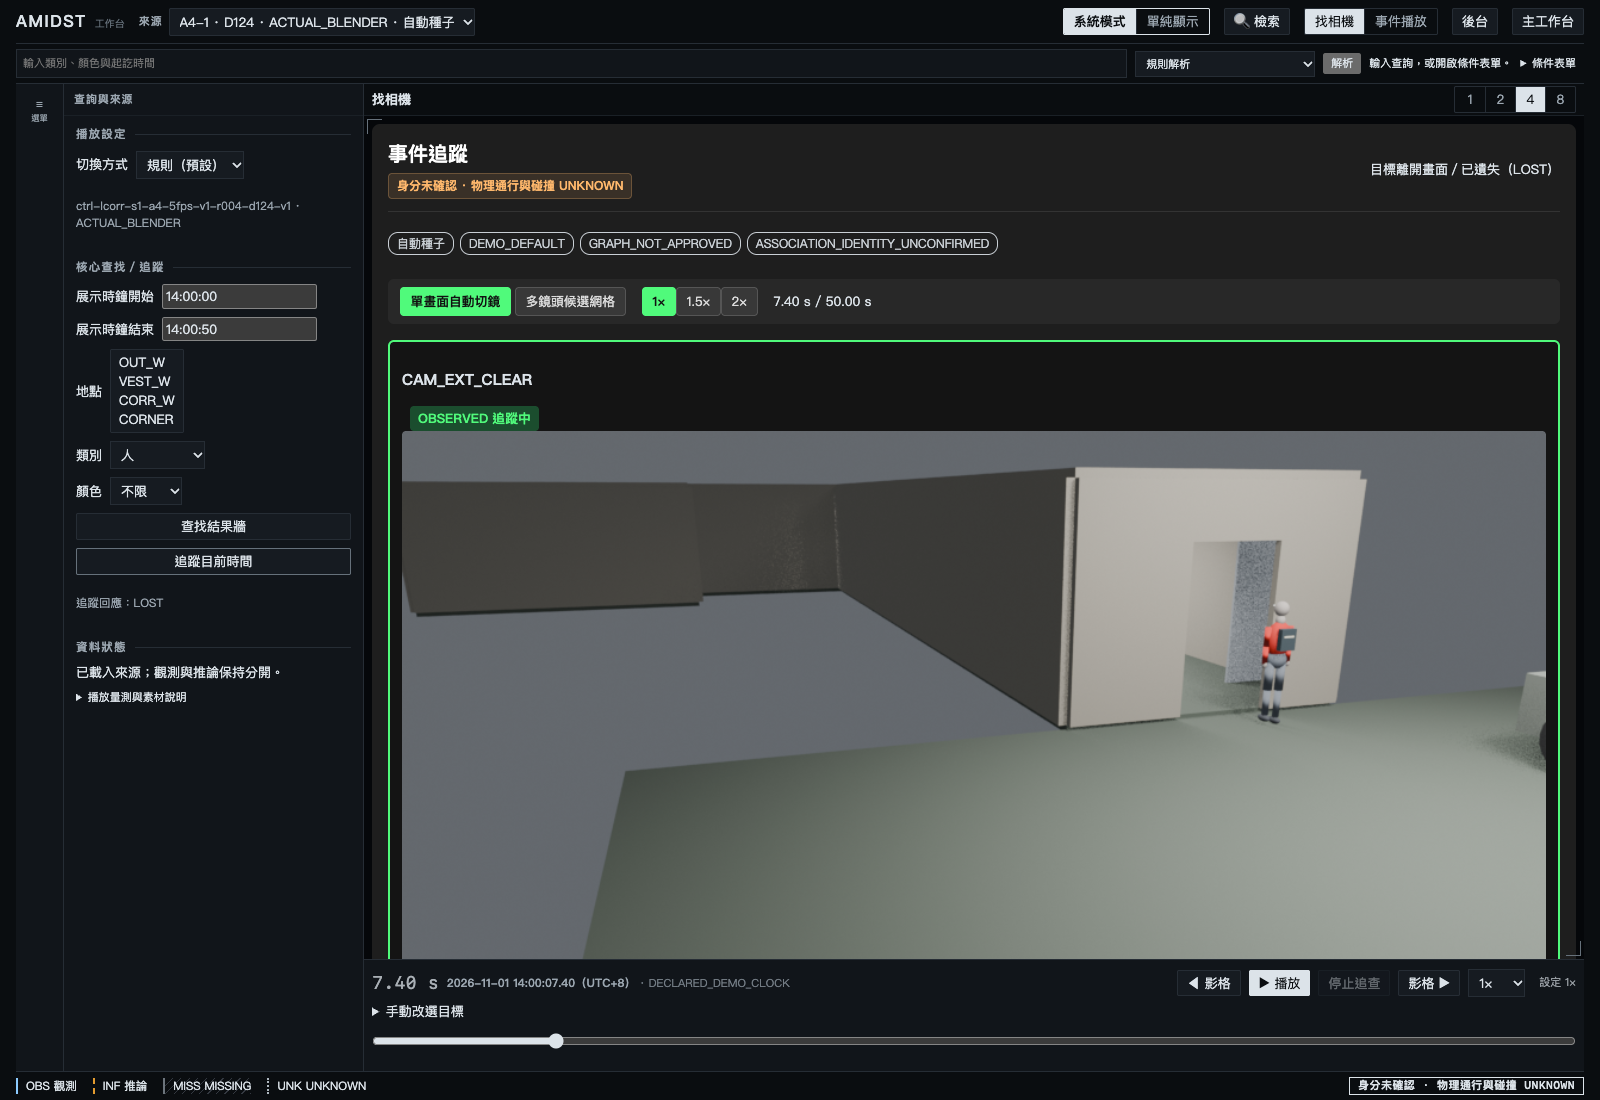
\includegraphics[width=\linewidth]{figures/screen_a4_track_single.png}\\
  \footnotesize (a) A4-1 追蹤：單畫面自動切鏡，\code{OBSERVED} 追蹤中
\end{minipage}\hfill
\begin{minipage}{0.49\linewidth}\centering
  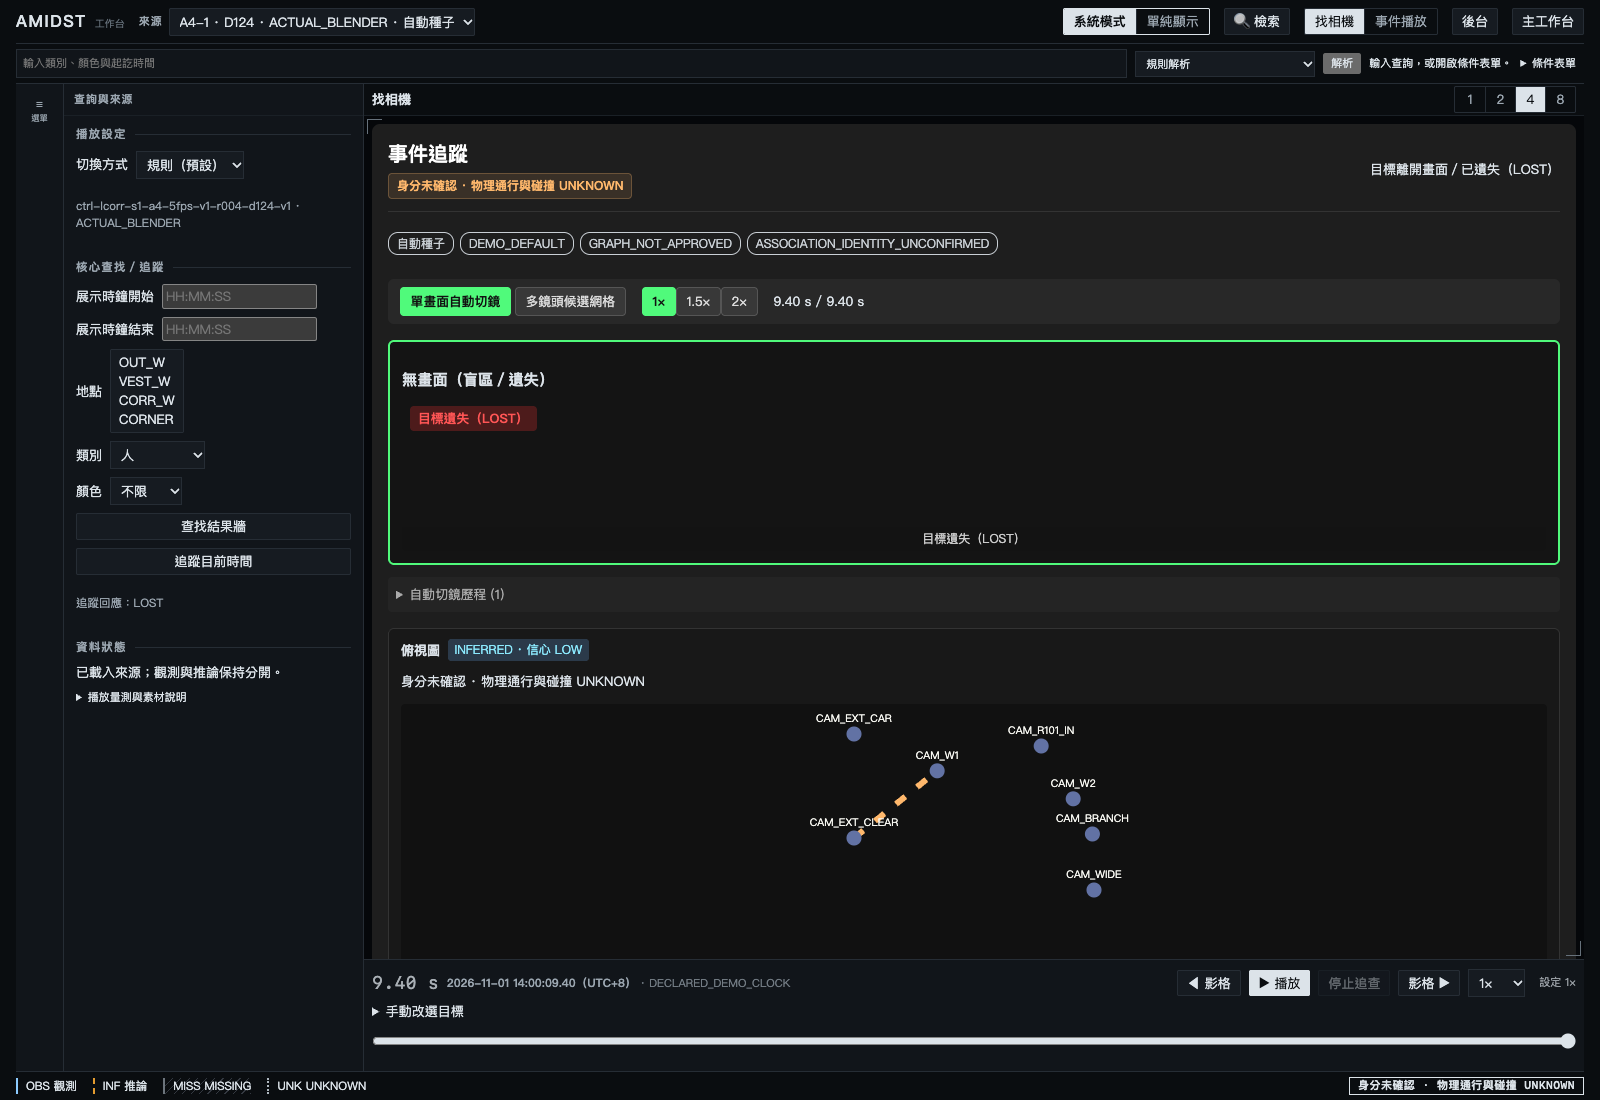
\includegraphics[width=\linewidth]{figures/screen_a4_blind.png}\\
  \footnotesize (b) A4-1 盲區：俯視圖 \code{INFERRED}、信心 \code{LOW} 的推測虛線
\end{minipage}\\[3mm]
\begin{minipage}{0.62\linewidth}\centering
  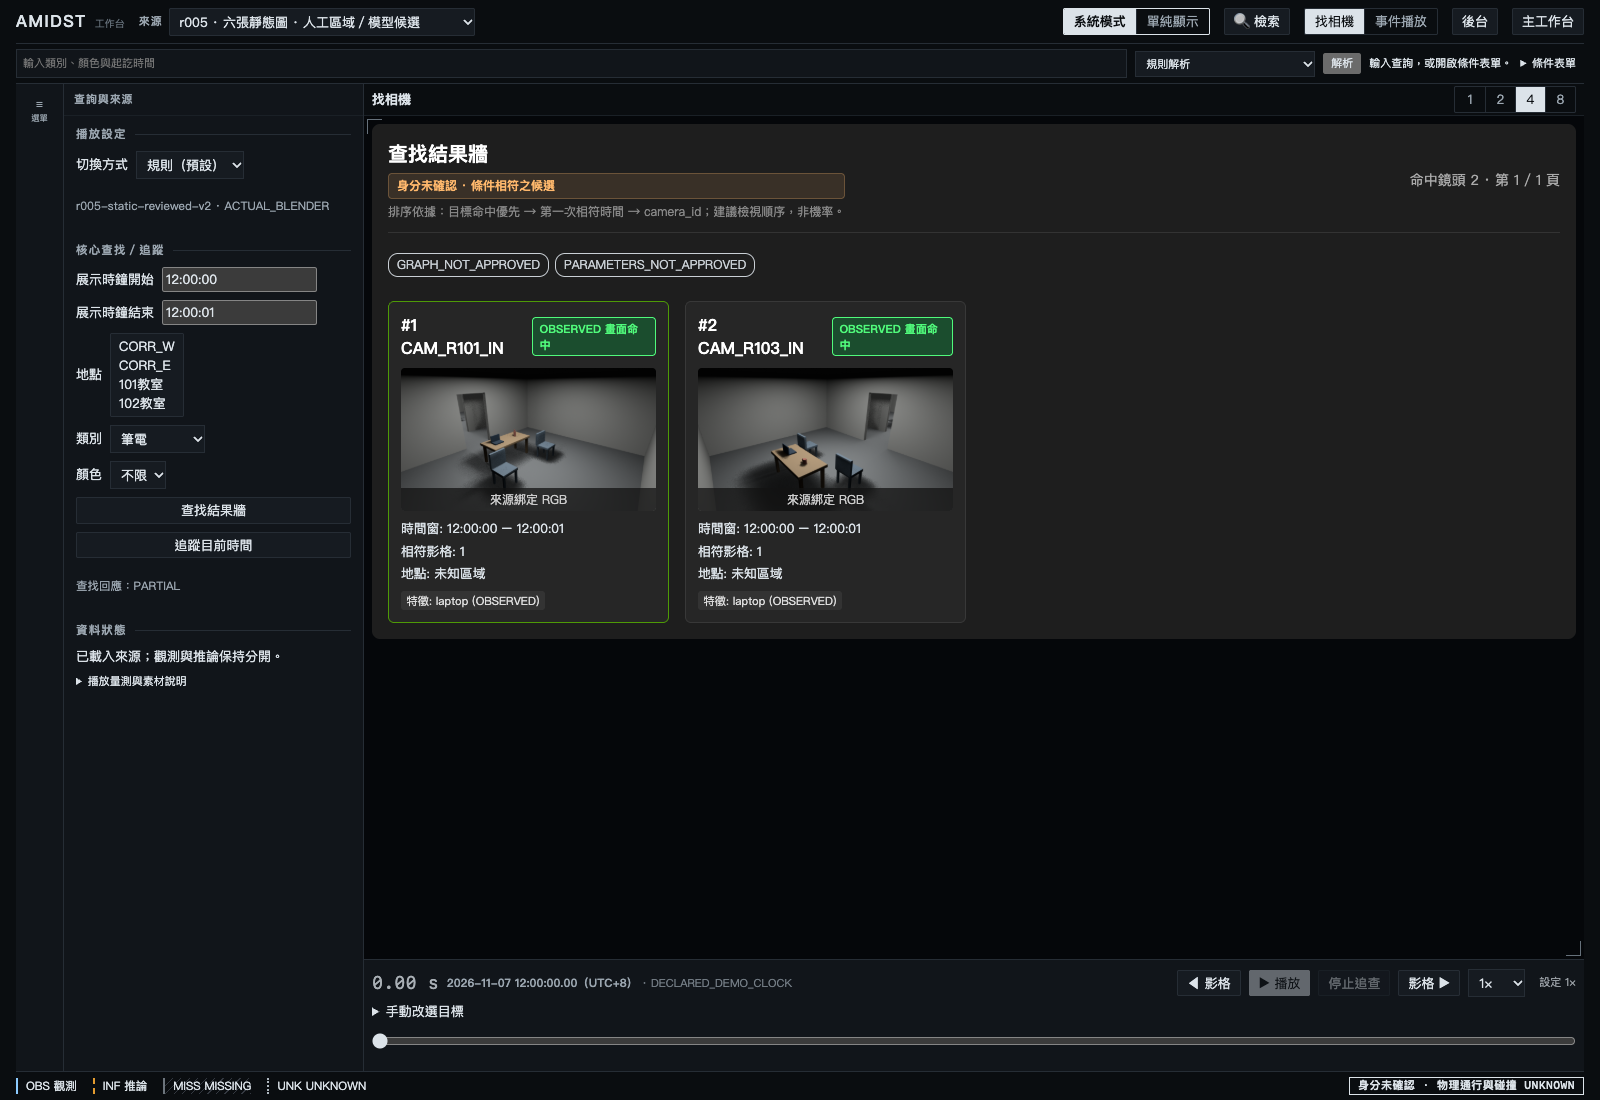
\includegraphics[width=\linewidth]{figures/screen_r005_search.png}\\
  \footnotesize (c) r005 查找結果牆：類別「筆電」命中 2 台鏡頭，回應 \code{PARTIAL}
\end{minipage}
\caption{實際畫面。所有畫面皆標示「身分未確認」；(a)(b) 帶 \code{DEMO_DEFAULT}、\code{GRAPH_NOT_APPROVED} 等原因碼晶片。}
\label{fig:screens}
\end{figure}

%=====================================================================
\section{討論與限制}\label{sec:discussion}
\subsection{Agentic 程度的客觀評估}
系統副標題為「Agentic 驅動」，但目前的證據不支持這個說法：
\begin{itemize}
  \item \textbf{所有自主行為都是規則或演算法。}自動換鏡頭是契約 §3.5 的純函式規則\src{S5}；自動種子是固定 preset（person、無顏色、無區域）\src{S1}；盲區推測是 \eqref{eq:window} 的時間窗與顯示座標連線\src{S6}；查找流程是索引與圖的條件比對\src{S5}。
  \item \textbf{語言模型 Agent 模式不可用。}Qwen3 1.7B 在原時間預算下 18 次全部逾時\src{S3}；切鏡模式支援 \code{RULE_ONLY} 與 \code{AGENT_SEQUENTIAL}，Agent 失敗時退回規則\src{S7b}；實機畫面的切換方式為「規則（預設）」（圖~\ref{fig:screens}）。
  \item \textbf{OpenAI 介接預設關閉。}程式註明為俯視圖的「外部推測線」，預設關閉，不進入 Q1–Q5 決策、候選排序或評估計分\src{S7c}；接上後只產生顯示用的候選鏡頭與理由。
\end{itemize}
結論：副標題中的「Agentic」目前尚未被實際驗證。補上的方式有三：(1) 讓 Agent 在規則之上做出可量測的決策（例如盲區後的候選鏡頭排序或查詢改寫），並以 \code{RULE_ONLY} 為基準做對照實驗；(2) 把 Agent 的回應時間壓到預算內（較小模型、預先生成或批次化），並記錄逾時率；(3) 以 RQ3 的自然語言解析作為第一個有 Agent 參與、有正式指標的功能。若無法在報告前完成，建議把副標題改為描述實際能力的用語。

\subsection{其他限制}
\begin{itemize}
  \item \textbf{合成影像。}B-05 使用 P1 v4 \code{SYNTHETIC} RGB，只有 A4-1／B4-1 是 \code{ACTUAL_BLENDER} RGB\src{S1}；且 B-05 沒有可畫的盲區曲線\src{S1}。
  \item \textbf{身分未確認。}所有輸出為 \code{UNCONFIRMED}；A4 W1 的弱觀測可能是假陽性，仍只是假設\src{S1}；盲區虛線為 \code{DISPLAY_ONLY}，不證明身分或動線\src{S1}。
  \item \textbf{\code{DEMO_DEFAULT} 與未核定參數。}A4／B4 的區域圖與參數尚未正式核定（\code{GRAPH_NOT_APPROVED}、\code{PARTIAL}），r004 設定為 \code{PROPOSED_NOT_FROZEN}\src{S1,S8}；物理預測參數也只是 PROPOSED\src{S6}。
  \item \textbf{尚未量測的項目。}偵測與身分正確率、正式參數、物理通行／碰撞、實體螢幕 fps、Windows／Linux 皆未驗收\src{S1}；第 \ref{sec:latency} 節列出的延遲項目為 \NR。
  \item \textbf{歷史量測不在 r004。}表~\ref{tab:latency} 的數字來自工程場景，r004 實測後應取代\src{S3}。
\end{itemize}

%=====================================================================
\section{結論與後續}
本階段完成了 D126 兩個核心功能在 r004／r005、三個事件上的整合與功能驗收，自動化測試全數通過\src{S1,S2}；架構上以離線索引避開即時偵測所需的大量 worker（\EXT）\src{S3}，並以 GT 隔離與 fail-closed 規則確保畫面上只出現可追溯的證據。尚未完成的是研究問題的正式評估與 Agent 能力的驗證。後續工作：
\begin{enumerate}
  \item RQ4：取得 yyin 的正式標註後計算 precision／recall／F1。
  \item RQ3：完成 \#480 自然語言解析並評估。
  \item 依 \#479 補量 r004 逐張偵測時間（runner 需記錄逐張前向時間）、case1／case2 回應時間與切鏡延遲。
  \item 把盲區假設模組（\eqref{eq:reach}–\eqref{eq:admissible}）接入 case2，並在 A4／B4 上與 \eqref{eq:window} 的顯示路徑比較。
  \item 依第 \ref{sec:discussion} 節的方式驗證或修正「Agentic」的宣稱。
\end{enumerate}

%=====================================================================
\begin{thebibliography}{99}\small
\bibitem{aharon2022botsort} N. Aharon, R. Orfaig, and B.-Z. Bobrovsky, ``BoT-SORT: Robust Associations Multi-Pedestrian Tracking,'' arXiv:2206.14651, 2022.
\bibitem{chavdarova2018wildtrack} T. Chavdarova \emph{et al.}, ``WILDTRACK: A Multi-Camera HD Dataset for Dense Unscripted Pedestrian Detection,'' in \emph{Proc. CVPR}, pp. 5030--5039, 2018.（完整作者名單待核）
\bibitem{feng2021cityflownl} Q. Feng, V. Ablavsky, and S. Sclaroff, ``CityFlow-NL: Tracking and Retrieval of Vehicles at City Scale by Natural Language Descriptions,'' arXiv:2101.04741, 2021.
\bibitem{javed2003} O. Javed, Z. Rasheed, K. Shafique, and M. Shah, ``Tracking Across Multiple Cameras with Disjoint Views,'' in \emph{Proc. ICCV}, 2003.（頁次待核）
\bibitem{kettnaker1999} V. Kettnaker and R. Zabih, ``Bayesian Multi-Camera Surveillance,'' in \emph{Proc. CVPR}, 1999.（頁次待核）
\bibitem{lee_cltm} Y.-G. Lee, Z. Tang, J.-N. Hwang, and Z. Fang, ``Online-Learning-Based Human Tracking Across Non-Overlapping Cameras,'' \emph{IEEE Trans. Circuits Syst. Video Technol.}（卷期、頁次與年份待核；作者名單待核）
\bibitem{luo2021clip4clip} H. Luo \emph{et al.}, ``CLIP4Clip: An Empirical Study of CLIP for End to End Video Clip Retrieval,'' arXiv:2104.08860, 2021.（完整作者名單待核）
\bibitem{lv2023rtdetr} W. Lv \emph{et al.}, ``DETRs Beat YOLOs on Real-time Object Detection,'' arXiv:2304.08069, 2023.（正式會議版本與作者名單待核）
\bibitem{makris2004} D. Makris, T. Ellis, and J. Black, ``Bridging the Gaps Between Cameras,'' in \emph{Proc. CVPR}, pp. 205--210, 2004.
\bibitem{nvidia_mv3dt} NVIDIA, ``DeepStream SDK 8.0 Multi-View 3D Tracking (MV3DT),'' \url{https://archive.docs.nvidia.com/metropolis/deepstream/8.0/text/DS_MV3DT.html}.
\bibitem{nvidia_vss} NVIDIA, ``Blueprint for Video Search and Summarization (VSS) 3.0,'' \url{https://docs.nvidia.com/vss/3.0.0/overview/latest}.
\bibitem{ristani2016} E. Ristani, F. Solera, R. Zou, R. Cucchiara, and C. Tomasi, ``Performance Measures and a Data Set for Multi-Target, Multi-Camera Tracking,'' in \emph{ECCV Workshops}, LNCS 9914, pp. 17--35, 2016.
\bibitem{tang2025aic9} Z. Tang \emph{et al.}, ``The 9th AI City Challenge,'' in \emph{ICCV Workshops}, 2025.（頁次待核）
\bibitem{wang2024aic8} S. Wang \emph{et al.}, ``The 8th AI City Challenge,'' in \emph{CVPR Workshops}, 2024.（頁次待核）
\bibitem{zhang2022bytetrack} Y. Zhang \emph{et al.}, ``ByteTrack: Multi-Object Tracking by Associating Every Detection Box,'' in \emph{Proc. ECCV}, 2022.（頁次與作者名單待核）
\bibitem{zhou2019osnet} K. Zhou, Y. Yang, A. Cavallaro, and T. Xiang, ``Omni-Scale Feature Learning for Person Re-Identification,'' in \emph{Proc. ICCV}, 2019.（頁次待核）
\end{thebibliography}

%=====================================================================
\appendix
\renewcommand{\thesection}{\Alph{section}}
\section{來源對照}\label{app:sources}
\begin{longtable}{l >{\raggedright\arraybackslash}p{12.6cm}}
\toprule
標記 & 來源 \\
\midrule
\endhead
S1 & \#445 Codex 留言 6717335520（2026-11-08），\url{https://github.com/Polalalabear/amidst/issues/445\#issuecomment-6717335520} \\
S2 & PR \#487 描述「實際產出」，\url{https://github.com/Polalalabear/amidst/pull/487}（head \code{53953a8}） \\
S3 & Issue \#479 內文（W-A24 延遲分析），\url{https://github.com/Polalalabear/amidst/issues/479}；其原始來源為 \#397 §B-4、\#93 留言 6362295156／6417324746、\code{docs/engineering/QWEN3_UNTRUNCATED_DIAGNOSTIC_20261025.md} \\
S4 & \code{docs/engineering/d133_playback_latency_20261108.json}@\code{1fdc1a4}（硬體、版本、\code{playback_trials}、\code{not_measured}） \\
S5 & \code{docs/contracts/Q_CORE_SEARCH_TRACK_V1.md}@\code{1fdc1a4}（§0、§1、§2.2、§3.5、§3.6、§4） \\
S6 & \code{src/amidst/q1q5/physical_prediction.py}@\code{1fdc1a4}（\code{PredictionParams}、\code{_window}） \\
S7 & \code{src/amidst/blind_hypothesis/engine.py}、\code{pruning.py}@\code{1fdc1a4}（模組說明） \\
S7b & \code{src/amidst/q1q5/q5_agent.py}@\code{1fdc1a4}（\code{RULE_ONLY}／\code{AGENT_SEQUENTIAL}／\code{RULE_FALLBACK}） \\
S7c & \code{src/amidst/q1q5/openai_prediction.py}@\code{1fdc1a4}（模組說明、\code{enabled=False}） \\
S8 & \code{configs/q1q5/r004_production_v1.json}@\code{1fdc1a4} \\
S9 & \code{docs/operations/D134_445_MAC_INTEGRATION.md}@\code{1fdc1a4} \\
S10 & 專題報告初稿（Claude Docs），\url{https://claude.ai/artifact/B7oycBdnYfkeK1U1JiPWSL}，第二章與參考文獻（2026-11-08 讀取，rev 11） \\
S11 & \#479 留言 6717580954（量測 A：離線偵測速度），\url{https://github.com/Polalalabear/amidst/issues/479\#issuecomment-6717580954}；原始數據 \code{docs/engineering/D131_417_DEMO_DEFAULT_RESULTS.md}／\code{.json}@\code{a786bde} \\
S12 & PR \#487 審查留言 6717576841（ADOPT、無 P1），\url{https://github.com/Polalalabear/amidst/pull/487\#issuecomment-6717576841} \\
\bottomrule
\end{longtable}

\section{分支、PR 與重現指令}
\begin{table}[htbp]
\centering\small
\caption{本紀錄引用的分支與 PR（2026-11-08 以 \code{gh pr view} 讀取）。}
\begin{tabular}{l l l l}
\toprule
PR & 分支 & head SHA & 狀態 \\
\midrule
\#485 & \code{claude/445-demo-integration} & \code{1fdc1a4da9824e8bd6230c1dbcd3a845ad869deb} & Draft \\
\#487 & \code{claude/ui-redesign-v1} & \code{53953a81e9194a5225832a59b38702b556c7a5de} & Draft \\
\#410 & \code{claude/core-search-track-contract} & \code{b1a619d0128450f03ace0002d7d1a5347355d02f} & Draft \\
\#484 & \code{claude/ui-redesign-spec} & \code{e3fdc1cf8377f97119bf48af3a83c7372a528d1e} & Draft \\
\#476 & \code{codex/459-mac-core-e2e} & \code{398cdbdd4af8165bbfe48229b5b3554022038daf} & Draft \\
\bottomrule
\end{tabular}
\end{table}

\noindent 重現指令（取自 S1；Python 環境路徑為原執行機器的本機路徑）：
\begin{small}
\begin{verbatim}
AMIDST_REQUIRE_IMPL=1 PYTHONPATH=src python -m pytest -o addopts= -q \
  tests/q1q5/test_core_search_track_t.py tests/q1q5/test_scene_graphs.py
AMIDST_REQUIRE_IMPL=1 node --test frontend/workbench-v2/*.test.mjs \
  frontend/event-viewer/*.test.mjs
node tests/browser/core-preview/core-e2e.mjs     # needs playwright-core, Chrome
node tests/browser/core-preview/real-e2e.mjs     # needs LOCAL RGB sources
python -B scripts/check_architecture_guard.py \
  --base 796cc176cd40bedbfe701b95192d3c8679755aa9
\end{verbatim}
\end{small}
本紀錄本身的編譯：\code{docs/research/experiment_record/build.sh}。

\end{document}
